% Created by tikzDevice version 0.12 on 2019-01-03 18:27:32
% !TEX encoding = UTF-8 Unicode
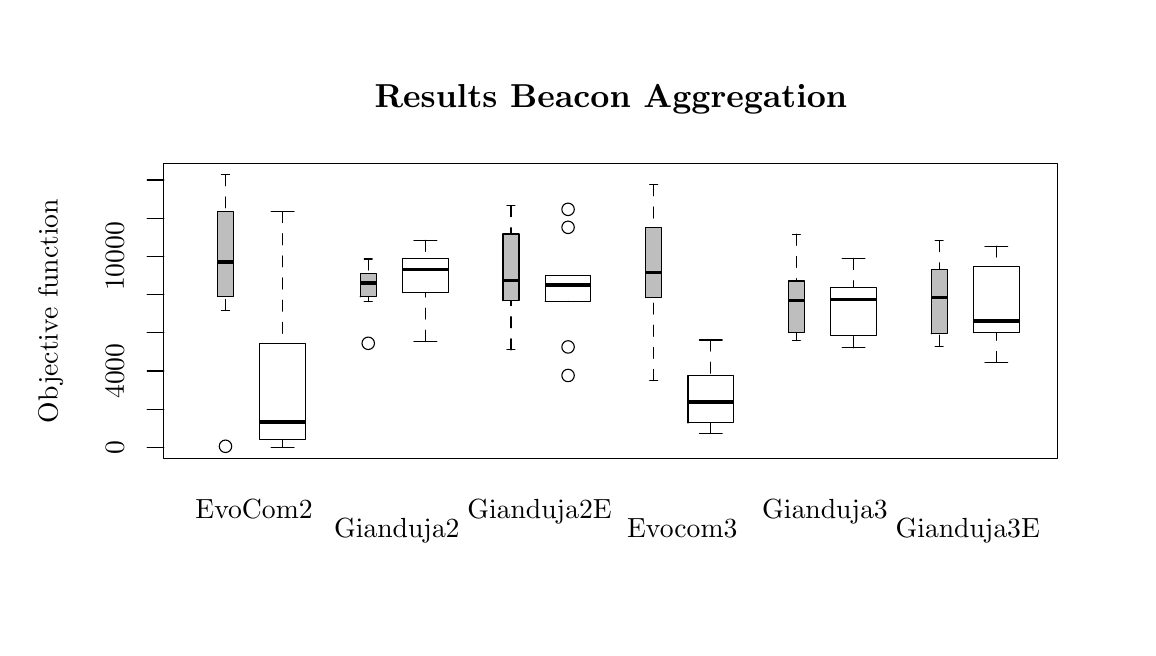
\begin{tikzpicture}[x=1pt,y=1pt]
\definecolor{fillColor}{RGB}{255,255,255}
\path[use as bounding box,fill=fillColor,fill opacity=0.00] (0,0) rectangle (397.48,216.81);
\begin{scope}
\path[clip] ( 49.20, 61.20) rectangle (372.28,167.61);
\definecolor{fillColor}{RGB}{190,190,190}

\path[fill=fillColor] ( 68.59,119.69) --
	( 74.37,119.69) --
	( 74.37,150.30) --
	( 68.59,150.30) --
	cycle;
\definecolor{drawColor}{RGB}{0,0,0}

\path[draw=drawColor,line width= 1.2pt,line join=round] ( 68.59,132.16) -- ( 74.37,132.16);

\path[draw=drawColor,line width= 0.4pt,dash pattern=on 4pt off 4pt ,line join=round,line cap=round] ( 71.48,114.65) -- ( 71.48,119.69);

\path[draw=drawColor,line width= 0.4pt,dash pattern=on 4pt off 4pt ,line join=round,line cap=round] ( 71.48,163.67) -- ( 71.48,150.30);

\path[draw=drawColor,line width= 0.4pt,line join=round,line cap=round] ( 70.04,114.65) -- ( 72.93,114.65);

\path[draw=drawColor,line width= 0.4pt,line join=round,line cap=round] ( 70.04,163.67) -- ( 72.93,163.67);

\path[draw=drawColor,line width= 0.4pt,line join=round,line cap=round] ( 68.59,119.69) --
	( 74.37,119.69) --
	( 74.37,150.30) --
	( 68.59,150.30) --
	( 68.59,119.69);

\path[draw=drawColor,line width= 0.4pt,line join=round,line cap=round] ( 71.48, 65.55) circle (  2.25);
\definecolor{fillColor}{RGB}{255,255,255}

\path[fill=fillColor] ( 83.86, 68.02) --
	(100.37, 68.02) --
	(100.37,102.82) --
	( 83.86,102.82) --
	cycle;

\path[draw=drawColor,line width= 1.2pt,line join=round] ( 83.86, 74.31) -- (100.37, 74.31);

\path[draw=drawColor,line width= 0.4pt,dash pattern=on 4pt off 4pt ,line join=round,line cap=round] ( 92.11, 65.14) -- ( 92.11, 68.02);

\path[draw=drawColor,line width= 0.4pt,dash pattern=on 4pt off 4pt ,line join=round,line cap=round] ( 92.11,150.35) -- ( 92.11,102.82);

\path[draw=drawColor,line width= 0.4pt,line join=round,line cap=round] ( 87.99, 65.14) -- ( 96.24, 65.14);

\path[draw=drawColor,line width= 0.4pt,line join=round,line cap=round] ( 87.99,150.35) -- ( 96.24,150.35);

\path[draw=drawColor,line width= 0.4pt,line join=round,line cap=round] ( 83.86, 68.02) --
	(100.37, 68.02) --
	(100.37,102.82) --
	( 83.86,102.82) --
	( 83.86, 68.02);
\definecolor{fillColor}{RGB}{190,190,190}

\path[fill=fillColor] (120.17,119.58) --
	(125.95,119.58) --
	(125.95,128.09) --
	(120.17,128.09) --
	cycle;

\path[draw=drawColor,line width= 1.2pt,line join=round] (120.17,124.60) -- (125.95,124.60);

\path[draw=drawColor,line width= 0.4pt,dash pattern=on 4pt off 4pt ,line join=round,line cap=round] (123.06,117.79) -- (123.06,119.58);

\path[draw=drawColor,line width= 0.4pt,dash pattern=on 4pt off 4pt ,line join=round,line cap=round] (123.06,133.20) -- (123.06,128.09);

\path[draw=drawColor,line width= 0.4pt,line join=round,line cap=round] (121.62,117.79) -- (124.50,117.79);

\path[draw=drawColor,line width= 0.4pt,line join=round,line cap=round] (121.62,133.20) -- (124.50,133.20);

\path[draw=drawColor,line width= 0.4pt,line join=round,line cap=round] (120.17,119.58) --
	(125.95,119.58) --
	(125.95,128.09) --
	(120.17,128.09) --
	(120.17,119.58);

\path[draw=drawColor,line width= 0.4pt,line join=round,line cap=round] (123.06,102.76) circle (  2.25);
\definecolor{fillColor}{RGB}{255,255,255}

\path[fill=fillColor] (135.44,121.10) --
	(151.94,121.10) --
	(151.94,133.54) --
	(135.44,133.54) --
	cycle;

\path[draw=drawColor,line width= 1.2pt,line join=round] (135.44,129.46) -- (151.94,129.46);

\path[draw=drawColor,line width= 0.4pt,dash pattern=on 4pt off 4pt ,line join=round,line cap=round] (143.69,103.47) -- (143.69,121.10);

\path[draw=drawColor,line width= 0.4pt,dash pattern=on 4pt off 4pt ,line join=round,line cap=round] (143.69,139.98) -- (143.69,133.54);

\path[draw=drawColor,line width= 0.4pt,line join=round,line cap=round] (139.56,103.47) -- (147.82,103.47);

\path[draw=drawColor,line width= 0.4pt,line join=round,line cap=round] (139.56,139.98) -- (147.82,139.98);

\path[draw=drawColor,line width= 0.4pt,line join=round,line cap=round] (135.44,121.10) --
	(151.94,121.10) --
	(151.94,133.54) --
	(135.44,133.54) --
	(135.44,121.10);
\definecolor{fillColor}{RGB}{190,190,190}

\path[fill=fillColor] (171.75,118.19) --
	(177.53,118.19) --
	(177.53,142.24) --
	(171.75,142.24) --
	cycle;

\path[draw=drawColor,line width= 1.2pt,line join=round] (171.75,125.36) -- (177.53,125.36);

\path[draw=drawColor,line width= 0.4pt,dash pattern=on 4pt off 4pt ,line join=round,line cap=round] (174.64,100.36) -- (174.64,118.19);

\path[draw=drawColor,line width= 0.4pt,dash pattern=on 4pt off 4pt ,line join=round,line cap=round] (174.64,152.51) -- (174.64,142.24);

\path[draw=drawColor,line width= 0.4pt,line join=round,line cap=round] (173.19,100.36) -- (176.08,100.36);

\path[draw=drawColor,line width= 0.4pt,line join=round,line cap=round] (173.19,152.51) -- (176.08,152.51);

\path[draw=drawColor,line width= 0.4pt,line join=round,line cap=round] (171.75,118.19) --
	(177.53,118.19) --
	(177.53,142.24) --
	(171.75,142.24) --
	(171.75,118.19);
\definecolor{fillColor}{RGB}{255,255,255}

\path[fill=fillColor] (187.02,117.94) --
	(203.52,117.94) --
	(203.52,127.28) --
	(187.02,127.28) --
	cycle;

\path[draw=drawColor,line width= 1.2pt,line join=round] (187.02,123.86) -- (203.52,123.86);

\path[draw=drawColor,line width= 0.4pt,dash pattern=on 4pt off 4pt ,line join=round,line cap=round] (195.27,117.94) -- (195.27,117.94);

\path[draw=drawColor,line width= 0.4pt,dash pattern=on 4pt off 4pt ,line join=round,line cap=round] (195.27,127.28) -- (195.27,127.28);

\path[draw=drawColor,line width= 0.4pt,line join=round,line cap=round] (191.14,117.94) -- (199.40,117.94);

\path[draw=drawColor,line width= 0.4pt,line join=round,line cap=round] (191.14,127.28) -- (199.40,127.28);

\path[draw=drawColor,line width= 0.4pt,line join=round,line cap=round] (187.02,117.94) --
	(203.52,117.94) --
	(203.52,127.28) --
	(187.02,127.28) --
	(187.02,117.94);

\path[draw=drawColor,line width= 0.4pt,line join=round,line cap=round] (195.27,151.16) circle (  2.25);

\path[draw=drawColor,line width= 0.4pt,line join=round,line cap=round] (195.27, 91.13) circle (  2.25);

\path[draw=drawColor,line width= 0.4pt,line join=round,line cap=round] (195.27,144.66) circle (  2.25);

\path[draw=drawColor,line width= 0.4pt,line join=round,line cap=round] (195.27,101.44) circle (  2.25);
\definecolor{fillColor}{RGB}{190,190,190}

\path[fill=fillColor] (223.33,119.28) --
	(229.10,119.28) --
	(229.10,144.69) --
	(223.33,144.69) --
	cycle;

\path[draw=drawColor,line width= 1.2pt,line join=round] (223.33,128.23) -- (229.10,128.23);

\path[draw=drawColor,line width= 0.4pt,dash pattern=on 4pt off 4pt ,line join=round,line cap=round] (226.22, 89.29) -- (226.22,119.28);

\path[draw=drawColor,line width= 0.4pt,dash pattern=on 4pt off 4pt ,line join=round,line cap=round] (226.22,160.03) -- (226.22,144.69);

\path[draw=drawColor,line width= 0.4pt,line join=round,line cap=round] (224.77, 89.29) -- (227.66, 89.29);

\path[draw=drawColor,line width= 0.4pt,line join=round,line cap=round] (224.77,160.03) -- (227.66,160.03);

\path[draw=drawColor,line width= 0.4pt,line join=round,line cap=round] (223.33,119.28) --
	(229.10,119.28) --
	(229.10,144.69) --
	(223.33,144.69) --
	(223.33,119.28);
\definecolor{fillColor}{RGB}{255,255,255}

\path[fill=fillColor] (238.59, 73.99) --
	(255.10, 73.99) --
	(255.10, 91.08) --
	(238.59, 91.08) --
	cycle;

\path[draw=drawColor,line width= 1.2pt,line join=round] (238.59, 81.58) -- (255.10, 81.58);

\path[draw=drawColor,line width= 0.4pt,dash pattern=on 4pt off 4pt ,line join=round,line cap=round] (246.85, 70.10) -- (246.85, 73.99);

\path[draw=drawColor,line width= 0.4pt,dash pattern=on 4pt off 4pt ,line join=round,line cap=round] (246.85,103.95) -- (246.85, 91.08);

\path[draw=drawColor,line width= 0.4pt,line join=round,line cap=round] (242.72, 70.10) -- (250.97, 70.10);

\path[draw=drawColor,line width= 0.4pt,line join=round,line cap=round] (242.72,103.95) -- (250.97,103.95);

\path[draw=drawColor,line width= 0.4pt,line join=round,line cap=round] (238.59, 73.99) --
	(255.10, 73.99) --
	(255.10, 91.08) --
	(238.59, 91.08) --
	(238.59, 73.99);
\definecolor{fillColor}{RGB}{190,190,190}

\path[fill=fillColor] (274.91,106.64) --
	(280.68,106.64) --
	(280.68,125.28) --
	(274.91,125.28) --
	cycle;

\path[draw=drawColor,line width= 1.2pt,line join=round] (274.91,118.20) -- (280.68,118.20);

\path[draw=drawColor,line width= 0.4pt,dash pattern=on 4pt off 4pt ,line join=round,line cap=round] (277.79,103.76) -- (277.79,106.64);

\path[draw=drawColor,line width= 0.4pt,dash pattern=on 4pt off 4pt ,line join=round,line cap=round] (277.79,142.16) -- (277.79,125.28);

\path[draw=drawColor,line width= 0.4pt,line join=round,line cap=round] (276.35,103.76) -- (279.24,103.76);

\path[draw=drawColor,line width= 0.4pt,line join=round,line cap=round] (276.35,142.16) -- (279.24,142.16);

\path[draw=drawColor,line width= 0.4pt,line join=round,line cap=round] (274.91,106.64) --
	(280.68,106.64) --
	(280.68,125.28) --
	(274.91,125.28) --
	(274.91,106.64);
\definecolor{fillColor}{RGB}{255,255,255}

\path[fill=fillColor] (290.17,105.73) --
	(306.68,105.73) --
	(306.68,122.97) --
	(290.17,122.97) --
	cycle;

\path[draw=drawColor,line width= 1.2pt,line join=round] (290.17,118.59) -- (306.68,118.59);

\path[draw=drawColor,line width= 0.4pt,dash pattern=on 4pt off 4pt ,line join=round,line cap=round] (298.43,101.15) -- (298.43,105.73);

\path[draw=drawColor,line width= 0.4pt,dash pattern=on 4pt off 4pt ,line join=round,line cap=round] (298.43,133.43) -- (298.43,122.97);

\path[draw=drawColor,line width= 0.4pt,line join=round,line cap=round] (294.30,101.15) -- (302.55,101.15);

\path[draw=drawColor,line width= 0.4pt,line join=round,line cap=round] (294.30,133.43) -- (302.55,133.43);

\path[draw=drawColor,line width= 0.4pt,line join=round,line cap=round] (290.17,105.73) --
	(306.68,105.73) --
	(306.68,122.97) --
	(290.17,122.97) --
	(290.17,105.73);
\definecolor{fillColor}{RGB}{190,190,190}

\path[fill=fillColor] (326.48,106.14) --
	(332.26,106.14) --
	(332.26,129.45) --
	(326.48,129.45) --
	cycle;

\path[draw=drawColor,line width= 1.2pt,line join=round] (326.48,119.34) -- (332.26,119.34);

\path[draw=drawColor,line width= 0.4pt,dash pattern=on 4pt off 4pt ,line join=round,line cap=round] (329.37,101.72) -- (329.37,106.14);

\path[draw=drawColor,line width= 0.4pt,dash pattern=on 4pt off 4pt ,line join=round,line cap=round] (329.37,139.85) -- (329.37,129.45);

\path[draw=drawColor,line width= 0.4pt,line join=round,line cap=round] (327.93,101.72) -- (330.82,101.72);

\path[draw=drawColor,line width= 0.4pt,line join=round,line cap=round] (327.93,139.85) -- (330.82,139.85);

\path[draw=drawColor,line width= 0.4pt,line join=round,line cap=round] (326.48,106.14) --
	(332.26,106.14) --
	(332.26,129.45) --
	(326.48,129.45) --
	(326.48,106.14);
\definecolor{fillColor}{RGB}{255,255,255}

\path[fill=fillColor] (341.75,106.63) --
	(358.26,106.63) --
	(358.26,130.37) --
	(341.75,130.37) --
	cycle;

\path[draw=drawColor,line width= 1.2pt,line join=round] (341.75,110.85) -- (358.26,110.85);

\path[draw=drawColor,line width= 0.4pt,dash pattern=on 4pt off 4pt ,line join=round,line cap=round] (350.00, 95.85) -- (350.00,106.63);

\path[draw=drawColor,line width= 0.4pt,dash pattern=on 4pt off 4pt ,line join=round,line cap=round] (350.00,137.89) -- (350.00,130.37);

\path[draw=drawColor,line width= 0.4pt,line join=round,line cap=round] (345.88, 95.85) -- (354.13, 95.85);

\path[draw=drawColor,line width= 0.4pt,line join=round,line cap=round] (345.88,137.89) -- (354.13,137.89);

\path[draw=drawColor,line width= 0.4pt,line join=round,line cap=round] (341.75,106.63) --
	(358.26,106.63) --
	(358.26,130.37) --
	(341.75,130.37) --
	(341.75,106.63);
\end{scope}
\begin{scope}
\path[clip] (  0.00,  0.00) rectangle (397.48,216.81);
\definecolor{drawColor}{RGB}{0,0,0}

\node[text=drawColor,rotate= 90.00,anchor=base,inner sep=0pt, outer sep=0pt, scale=  1.00] at ( 10.80,114.41) {Objective function};
\end{scope}
\begin{scope}
\path[clip] (  0.00,  0.00) rectangle (397.48,216.81);
\definecolor{drawColor}{RGB}{0,0,0}

\node[text=drawColor,anchor=base,inner sep=0pt, outer sep=0pt, scale=  1.00] at ( 81.80, 39.60) {EvoCom2};

\node[text=drawColor,anchor=base,inner sep=0pt, outer sep=0pt, scale=  1.00] at (184.95, 39.60) {Gianduja2E};

\node[text=drawColor,anchor=base,inner sep=0pt, outer sep=0pt, scale=  1.00] at (288.11, 39.60) {Gianduja3};

\node[text=drawColor,anchor=base,inner sep=0pt, outer sep=0pt, scale=  1.00] at (133.38, 32.71) {Gianduja2};

\node[text=drawColor,anchor=base,inner sep=0pt, outer sep=0pt, scale=  1.00] at (236.53, 32.71) {Evocom3};

\node[text=drawColor,anchor=base,inner sep=0pt, outer sep=0pt, scale=  1.00] at (339.69, 32.71) {Gianduja3E};
\end{scope}
\begin{scope}
\path[clip] (  0.00,  0.00) rectangle (397.48,216.81);
\definecolor{drawColor}{RGB}{0,0,0}

\node[text=drawColor,anchor=base,inner sep=0pt, outer sep=0pt, scale=  1.20] at (210.74,188.07) {\bfseries Results Beacon Aggregation};
\end{scope}
\begin{scope}
\path[clip] (  0.00,  0.00) rectangle (397.48,216.81);
\definecolor{drawColor}{RGB}{0,0,0}

\path[draw=drawColor,line width= 0.4pt,line join=round,line cap=round] ( 49.20, 65.13) -- ( 49.20,161.77);

\path[draw=drawColor,line width= 0.4pt,line join=round,line cap=round] ( 49.20, 65.13) -- ( 43.20, 65.13);

\path[draw=drawColor,line width= 0.4pt,line join=round,line cap=round] ( 49.20, 78.94) -- ( 43.20, 78.94);

\path[draw=drawColor,line width= 0.4pt,line join=round,line cap=round] ( 49.20, 92.74) -- ( 43.20, 92.74);

\path[draw=drawColor,line width= 0.4pt,line join=round,line cap=round] ( 49.20,106.55) -- ( 43.20,106.55);

\path[draw=drawColor,line width= 0.4pt,line join=round,line cap=round] ( 49.20,120.36) -- ( 43.20,120.36);

\path[draw=drawColor,line width= 0.4pt,line join=round,line cap=round] ( 49.20,134.16) -- ( 43.20,134.16);

\path[draw=drawColor,line width= 0.4pt,line join=round,line cap=round] ( 49.20,147.97) -- ( 43.20,147.97);

\path[draw=drawColor,line width= 0.4pt,line join=round,line cap=round] ( 49.20,161.77) -- ( 43.20,161.77);

\node[text=drawColor,rotate= 90.00,anchor=base,inner sep=0pt, outer sep=0pt, scale=  1.00] at ( 34.80, 65.13) {0};

\node[text=drawColor,rotate= 90.00,anchor=base,inner sep=0pt, outer sep=0pt, scale=  1.00] at ( 34.80, 92.74) {4000};

\node[text=drawColor,rotate= 90.00,anchor=base,inner sep=0pt, outer sep=0pt, scale=  1.00] at ( 34.80,134.16) {10000};

\path[draw=drawColor,line width= 0.4pt,line join=round,line cap=round] ( 49.20, 61.20) --
	(372.28, 61.20) --
	(372.28,167.61) --
	( 49.20,167.61) --
	( 49.20, 61.20);
\end{scope}
\end{tikzpicture}
